\documentclass[border=8pt]{standalone}
\usepackage{tikz}
\usetikzlibrary{arrows.meta,positioning,calc}
\begin{document}
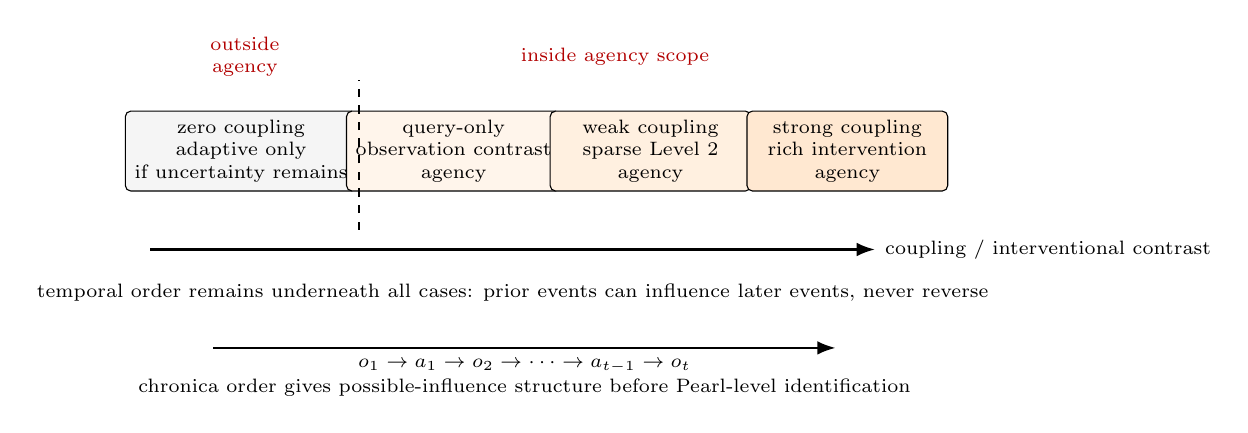
\begin{tikzpicture}[
  zone/.style={draw, rounded corners=2pt, align=center, minimum width=2.55cm, minimum height=1.0cm, font=\scriptsize},
  arr/.style={-Latex, thick},
  note/.style={align=center, font=\scriptsize}
]

\draw[arr] (0,0) -- (9.2,0) node[right, note] {coupling / interventional contrast};
\node[note] at (4.6,-0.55) {temporal order remains underneath all cases: prior events can influence later events, never reverse};

\node[zone, fill=gray!8, minimum width=2.85cm] (zero) at (1.15,1.25) {zero coupling\\adaptive only\\if uncertainty remains};
\node[zone, fill=orange!8] (query) at (3.85,1.25) {query-only\\observation contrast\\agency};
\node[zone, fill=orange!12] (weak) at (6.35,1.25) {weak coupling\\sparse Level 2\\agency};
\node[zone, fill=orange!18] (strong) at (8.85,1.25) {strong coupling\\rich intervention\\agency};

\draw[thick, dashed] (2.65,0.25) -- (2.65,2.15);
\node[note, red!70!black] at (1.2,2.45) {outside\\agency};
\node[note, red!70!black] at (5.9,2.45) {inside agency scope};

\draw[arr] (0.8,-1.25) -- node[below, note] {$o_1 \rightarrow a_1 \rightarrow o_2 \rightarrow \cdots \rightarrow a_{t-1} \rightarrow o_t$} (8.7,-1.25);
\node[note] at (4.75,-1.75) {chronica order gives possible-influence structure before Pearl-level identification};

\end{tikzpicture}
\end{document}
